\documentclass{article}
\usepackage{tikz}
\begin{document}

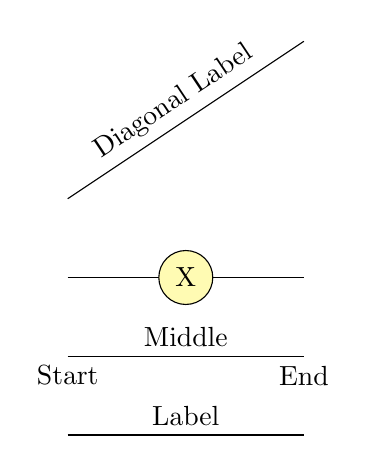
\begin{tikzpicture}[scale=1]

  % --- Simple path with inline node ---
  \draw (0,0) -- (3,0) node[midway, above] {Label};

  % --- Path with multiple inline nodes ---
  \draw (0,1) -- (3,1)
        node[pos=0, below] {Start}
        node[pos=0.5, above] {Middle}
        node[pos=1, below] {End};

  % --- Path with styled inline node ---
  \draw (0,2) -- (3,2)
        node[midway, draw, fill=yellow!30, circle] {X};

  % --- Diagonal path with sloped label above ---
  \draw (0,3) -- (3,5)
        node[midway, sloped, above] {Diagonal Label};

\end{tikzpicture}

\end{document}
